\documentclass[english]{report}
\usepackage{graphicx}
\usepackage{booktabs}
\usepackage{geometry}
\usepackage{hyperref}
\usepackage{babel}
\usepackage{lipsum}
\usepackage{subcaption}
\usepackage{float}
\usepackage{colortbl}

 \geometry{
 a4paper,
 total={170mm,257mm},
 left=20mm,
 top=20mm,
 }

\title{
    \leavevmode{
\includegraphics[width=1\textwidth]{../resources/img/polito_logo_2021_blu}\newline\newline}\\
     Fingerprint spoofing detection \\

}
\author{Riccardo Cardona, Nicholas Berardo}

\begin{document}

\maketitle

\chapter{Introduction}

\section{Abstract}
    The goal is to build the best model for the Fingerprint Spoofing Detection task, using the models developed during the 
    laboratory and the lessons.

\section{Overview}
    The data set and test set are composed of 10 dimensional features. The last column is the class label which is \textbf{1} for the \textit{authentic
    fingerprint} and \textbf{0} for the \textit{spoofed fingerprint}.\newline

    The datasets are imbalanced, we have more spoofed fingerprint then the authentic fingerprint. 
    The Training set is composed of ... samples and the Test set is composed of ... samples. \newline

    The application we are going to build has $\pi$ =0.5 meaning that we have the same prior probability for both classes, but we have different 
    costs. The cost of False Negative \textit{C\textsubscript{fn}} is 1 but the cost of False Positive
    \textit{C\textsubscript{fp}} is 10, so classifying a spoofed fingerprint as an authentic one
    has an higher cost due to security vulnerability.

\section{Features Analisys}
As we said, the Fingerprint Spoofing Detection task has 10 features. Here below we are going 
to analyze them.

\begin{figure}[h!]
    \begin{subfigure}{0.3\textwidth}
        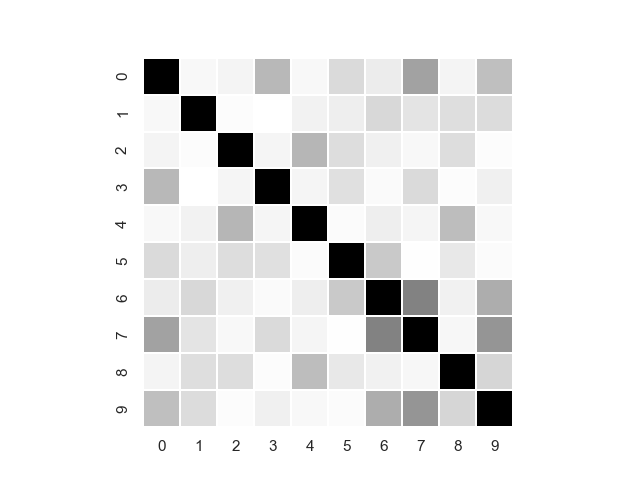
\includegraphics[scale=0.3]{../../images/feature_plot/heatmap_.png}
        \caption{All classes}
        
        \label{fig:heatmap}
    \end{subfigure}
    \begin{subfigure}{0.3\textwidth}
        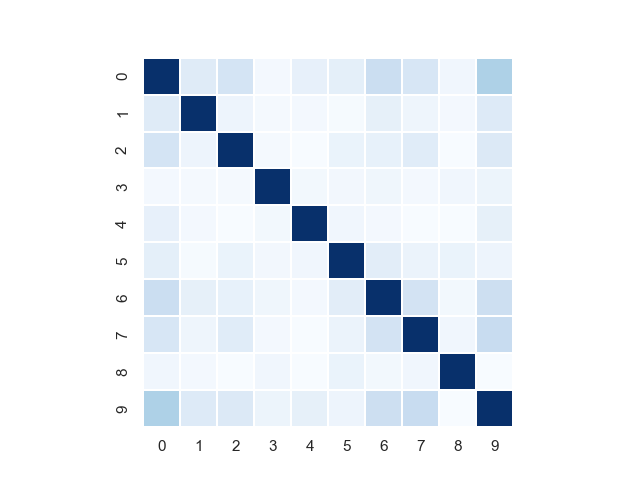
\includegraphics[scale=0.3]{../../images/feature_plot/heatmap_fingerprint_.png}
        \caption{Authentic Fingerprint}
        
        \label{fig:heatmap}
    \end{subfigure}
    \begin{subfigure}{0.3\textwidth}
        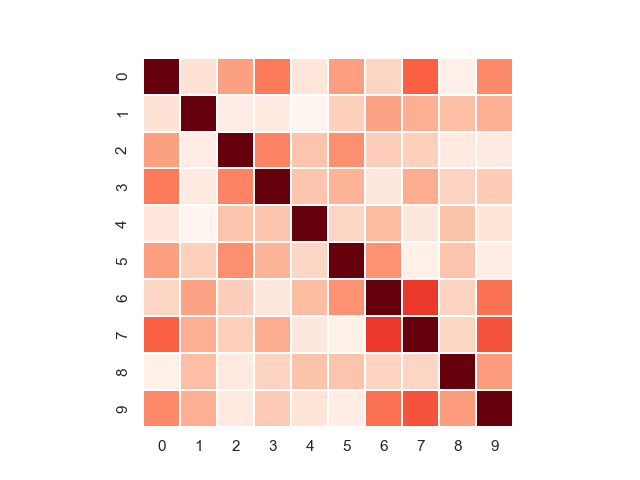
\includegraphics[scale=0.3]{../../images/feature_plot/heatmap_spoofedFingerprint_.png}
        \caption{Spoofed Fingerprint}
        
        \label{fig:heatmap}
    \end{subfigure}
    \centering
    \caption{Heatmap}
\end{figure}

As we can see from the Figures above, the correlation between the features is very small. 
This lead us to think that using PCA for dimensionality reduction is useless (it could
also remove some important information!), but we will try using it. \newline

Now we are going to see the histograms for each of the 10 features. It's easy to see that
each feature has a Gaussian distribution. \newline
\begin{figure}[h!]
    \begin{subfigure}{0.3\textwidth}
        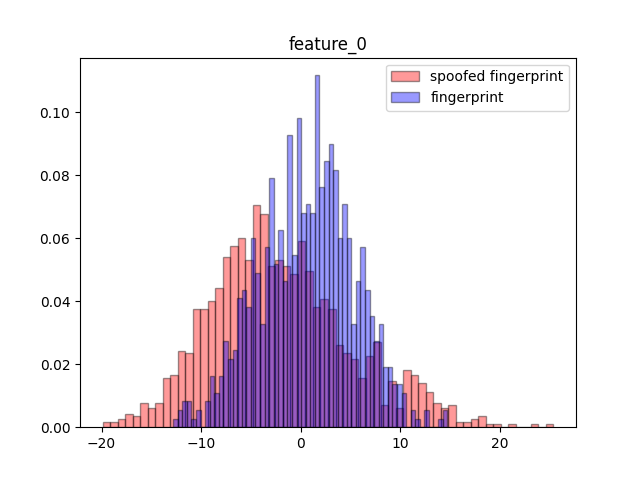
\includegraphics[scale=0.3]{../../images/feature_plot/hist_feature_0}
        \caption{RAW Feature 0}
    \end{subfigure}
    \begin{subfigure}{0.3\textwidth}
        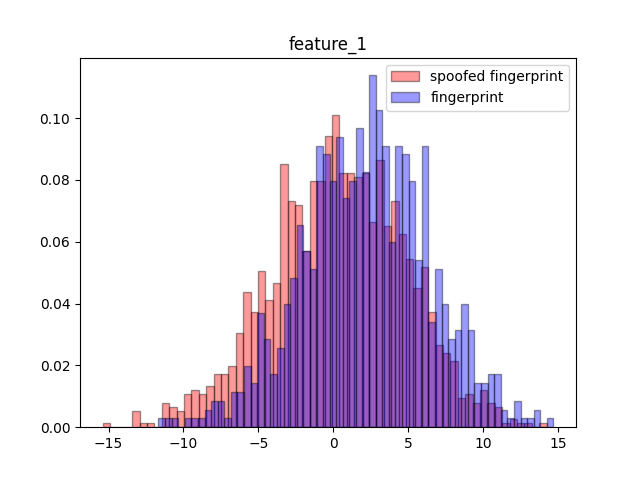
\includegraphics[scale=0.3]{../../images/feature_plot/hist_feature_1}
        \caption{RAW Feature 1}
    \end{subfigure}
    \begin{subfigure}{0.3\textwidth}
        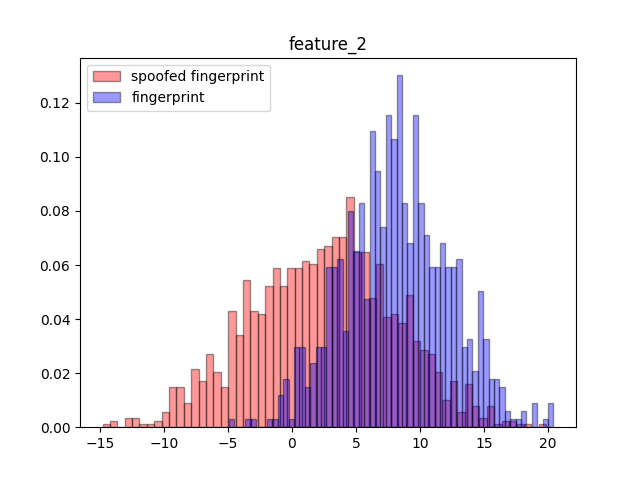
\includegraphics[scale=0.3]{../../images/feature_plot/hist_feature_2}
        \caption{RAW Feature 2}
    \end{subfigure}
    \begin{subfigure}{0.3\textwidth}
        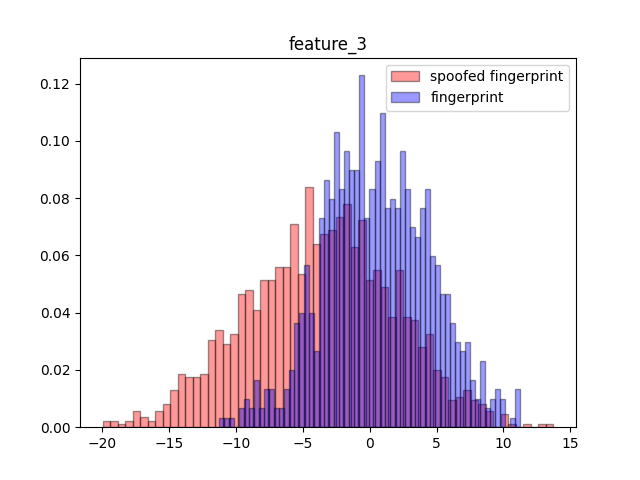
\includegraphics[scale=0.3]{../../images/feature_plot/hist_feature_3}
        \caption{RAW Feature 3}
    \end{subfigure}
    \begin{subfigure}{0.3\textwidth}
        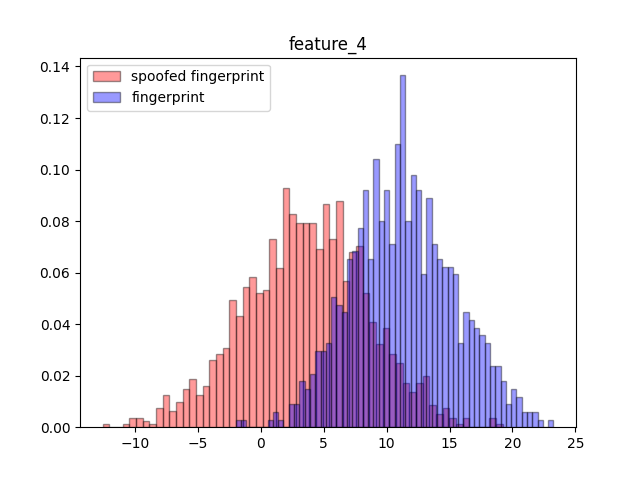
\includegraphics[scale=0.3]{../../images/feature_plot/hist_feature_4}
        \caption{RAW Feature 4}
    \end{subfigure}
    \begin{subfigure}{0.3\textwidth}
        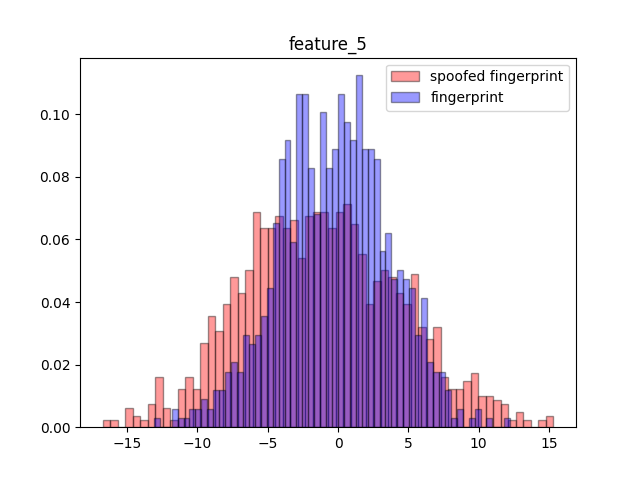
\includegraphics[scale=0.3]{../../images/feature_plot/hist_feature_5}
        \caption{RAW Feature 5}
    \end{subfigure}
    \begin{subfigure}{0.3\textwidth}
        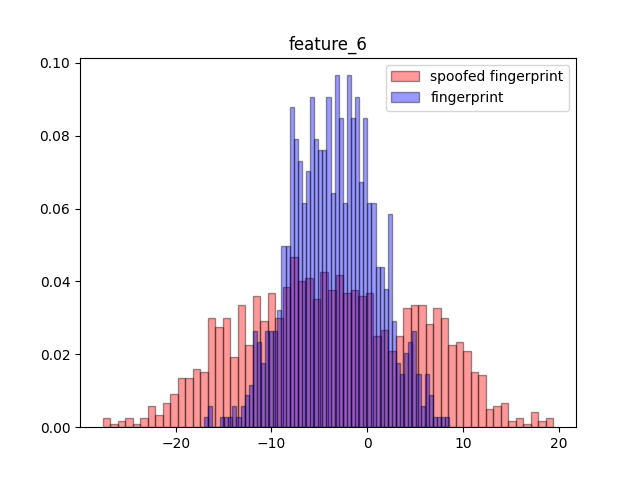
\includegraphics[scale=0.3]{../../images/feature_plot/hist_feature_6}
        \caption{RAW Feature 6}
    \end{subfigure}
    \begin{subfigure}{0.3\textwidth}
        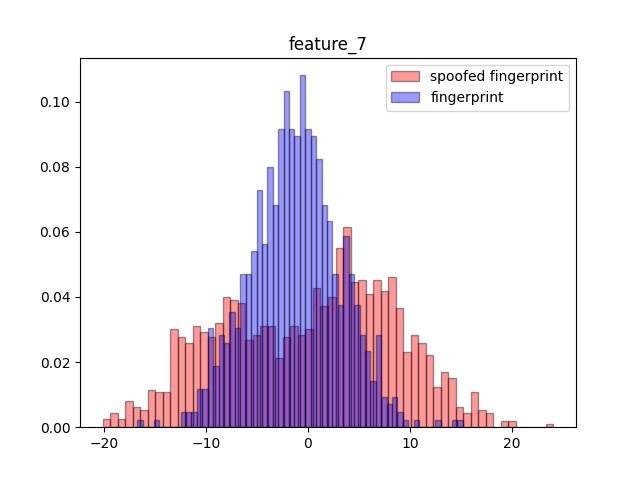
\includegraphics[scale=0.3]{../../images/feature_plot/hist_feature_7}
        \caption{RAW Feature 7}
    \end{subfigure}
    \begin{subfigure}{0.3\textwidth}
        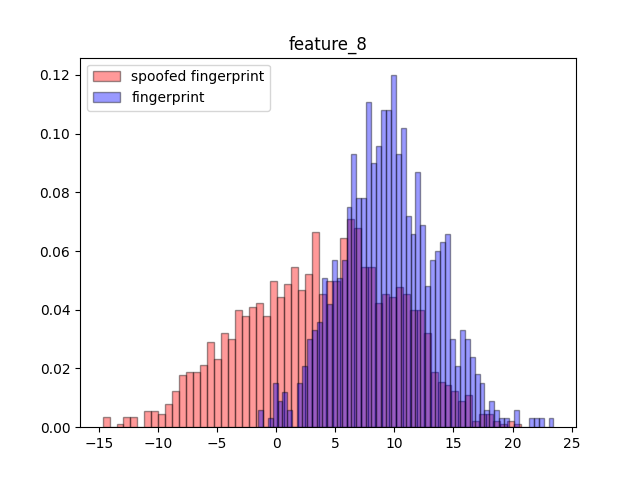
\includegraphics[scale=0.3]{../../images/feature_plot/hist_feature_8}
        \caption{RAW Feature 8}
    \end{subfigure}
    \begin{subfigure}{0.3\textwidth}
        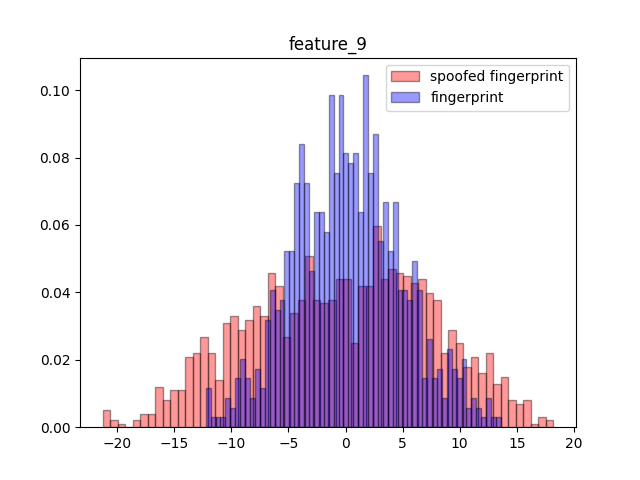
\includegraphics[scale=0.3]{../../images/feature_plot/hist_feature_9}
        \caption{RAW Feature 9}
    \end{subfigure}
    \centering
    \caption{RAW Feature Histogram}
\end{figure}



\section{PCA Usage}



    PCA (Principal Component Analysis) is a Dimensionality Reduction technique that can be used to
    remove noise, simplfy classification and data visualization. It can be also used to avoid overfitting,
    but it may produce underfitting if too many dimensions are removed (removing too many usefull 
    information). So it is a usefull technique but sometimes it can be useless because if used could
    lead only to bad models. \newline\newline
    What does PCA do? 

    First of all we need to compute the mean of the Dataset $\mu$, then we need to compute the covariance
    matrix 
    \[C = \frac{1}{K} \sum_{i=1}^{K} (x_i-\mu)(x_i-\mu)^T \]
    From C we need the eigen-decomposition \(C = U \Sigma U^T \), where U is a matrix that
    constains the eigen-vectors and $\Sigma$ is a diagonal matrix that contains the eigen-values
    in descending order.
    The solution are the \textit{m} eigen-vectors of U corresponding to the \textit{m} 
    highest eiget-values of $\Sigma$.


    \begin{figure}[H]
        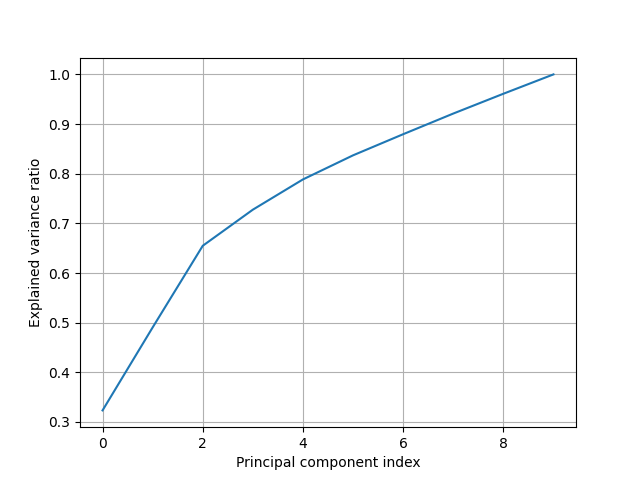
\includegraphics[scale=0.5]{../../images/feature_plot/PCA_explainedVariance.png}
        \centering
        \caption{PCA variance}
    \end{figure}
    As we can see, if we use 9 dimensions (Number 8 on the principal component index), we are going to
    reach a 96\% of explainance, then if we use 8 dimensions we will explain 91\% of the data variance.
    Starting from 7 to 1 dimensions, we are lower than 90\%. \newline
    We will consider only 9 and 8 as PCA parameter.

    \begin{figure}[H]
        \centering
        
        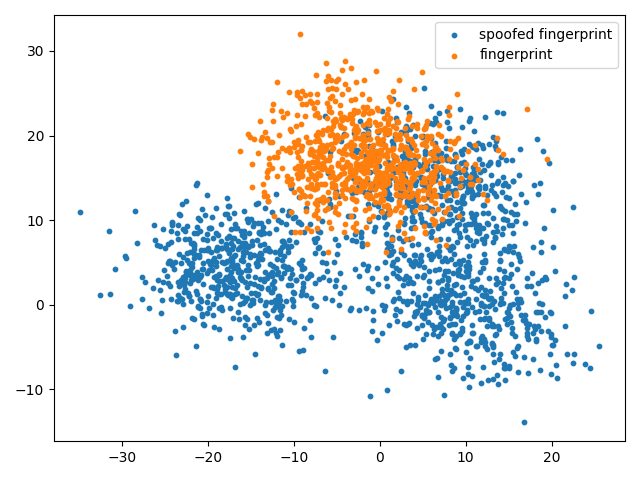
\includegraphics[scale=0.5]{../../images/feature_plot/PCA_m=2.png}
        \caption{PCA}
    \end{figure}

    From this plot (Figure 1.4) we can see the distribution of the 2 main features.

    \begin{figure}[H]
        \centering
        
        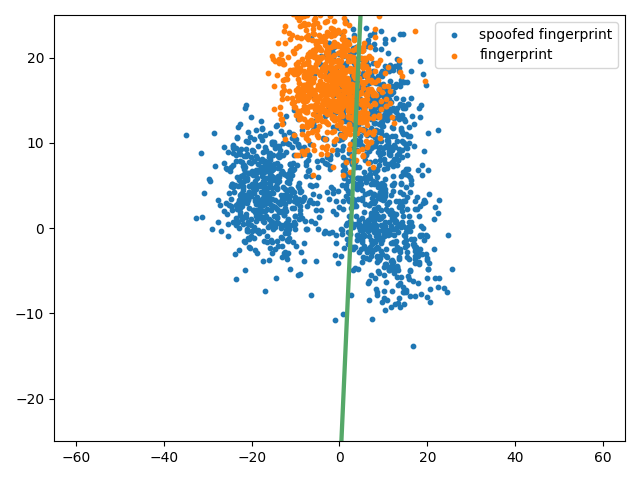
\includegraphics[scale=0.5]{../../images/feature_plot/PCA_m=2 + LDA.png}
        \caption{LDA}
    \end{figure}

    From this plot (Figure 1.5) we can see the distribution of the 2 main features using both PCA and LDA

\section{Training}
    \begin{itemize}
        \item We are going to use a K-Fold Cross Validation approach, with K = 5
        \item The minDCF computation is computed based on our application ($\pi$,C\textsubscript{fn},C\textsubscript{fp}) = (0.5,1,10), but we have
        computed the effective prior, which is approximated to ($\pi$,C\textsubscript{fn},C\textsubscript{fp}) = (0.09,1,1).\newline
        We have also tried this two different application:
        \begin{itemize}
            \item ($\pi$,C\textsubscript{fn},C\textsubscript{fp}) = (0.1,1,1)
            \item ($\pi$,C\textsubscript{fn},C\textsubscript{fp}) = (0.9,1,1)
        \end{itemize}
    \end{itemize}

\chapter{Classification and Validation}

\section{Introduction}
We are going to develop this following models:
\begin{itemize}
    \item Generative Models
    \begin{itemize}
        \item Multivariate Gaussian Classifier (\textbf{MVG})
        \item MVG Tied Covariance (Only one covariance matrix for everything)
        \item MVG Naive (For each covariance matrix takes out only the diagonal)
        \item MVG Tied Naive (Only one covariance matrix, but taking only the diagonal)
    \end{itemize}
    \item Logistic Regression (\textbf{LR})
    \begin{itemize}
        \item Linear Logistic Regression
        \item Quadratic Logistic Regression
    \end{itemize}
    \item Support Vector Machine (\textbf{SVM})
    \begin{itemize}
        \item \dots
    \end{itemize}
    \item Gaussian Mixture Models (\textbf{GMM})
    \begin{itemize}
        \item \dots
        \item \dots
    \end{itemize}
\end{itemize}

\clearpage

\section{Multivariate Gaussian Classifiers}

We are going to analyze all the Gaussian Classifiers, using the Multivariate Gaussian Classifier and all it's variants: 
\begin{itemize}
    \item Tied Covariance
    \item Naive Bayes
    \item Tied Naive Bayes
\end{itemize}

For all these 4 model we have 2 parameters: $\theta$ = ($\mu$, $\Sigma$). We can easily estimate them starting 
from the likelihood w.r.t. $\theta$ for the \textbf{M.V.G.}
\[ \mathcal{L} (\theta) = \prod_{c}^{K}\prod_{i|c_i=c} \mathcal{N} (x_i|\mu_c,\Sigma_c)\]
Then we can build the log-likelihood because it's easier to work with.
\[ l (\theta) = \sum_{c}^{K}\sum_{i|c_i=c} log \mathcal{N} (x_i|\mu_c,\Sigma_c)\]
Now we define \( l_c (\theta) = \sum_{i|c_i=c} log \mathcal{N} (x_i|\mu_c,\Sigma_c)\) and compute 
the $\nabla_\mu l_c(\mu_c,\Sigma_c) = 0$ and the $\nabla_\Sigma l_c(\mu_c,\Sigma_c) = 0$ 
obtaining 
\[\mu_c^* = \frac{1}{N_c}\sum_{i|c_i=c}x_i\] 
\[\Sigma_c^* = \frac{1}{N_c}\sum_{i|c_i=c}(x_i-\mu_c^*)(x_i-\mu_c^*)^T\] 

We can do the same thing for the \textbf{Naive Bayes} model (that has diagonal covariance matrix)
\[ l (\theta) = \sum_{c}^{K}\sum_{i|c_i=c}\sum_{j=1}^{D} log \mathcal{N} (x_{i,[j]}|\mu_{c,[j]},\Sigma_{c,[j]})\]
which solutions are
\[\mu_{c,[j]}^* = \frac{1}{N_c}\sum_{i|c_i=c}x_{i,[j]}\] 
\[\Sigma_{c,[j]}^* = \frac{1}{N_c}\sum_{i|c_i=c}(x_{i,[j]}-\mu_{c,[j]}^*)(x_{i,[j]}-\mu_{c,[j]}^*)^T\] 

Finally, the \textbf{Tied} model can be built in the same way (has a single covariance matrix for all classes)
\[ l (\theta) = \sum_{c}^{K}\sum_{i|c_i=c} log \mathcal{N} (x_i|\mu_c,\Sigma)\]
which solutions are
\[\mu_{c}^* = \frac{1}{N_c}\sum_{i|c_i=c}x_{i}\] 
\[\Sigma^* = \frac{1}{N}\sum_{c}^{K}\sum_{i|c_i=c}(x_{i}-\mu_{c}^*)(x_{i}-\mu_{c}^*)^T\] 

The tables below show the computation of the minDCF on the validation set (extracted using K-Fold Cross Validation with K = 5).
As said before we are going to consider the main application (0.5,1,10) and 2 other applications (0.1,1,1) and (0.9,1,1).
There are also some computation of PCA with m=9 and m=8.

\begin{table}[H]
    \centering
    \begin{tabular}{@{}llll@{}}
    \toprule
    Classifier          & pi = 0.1  & pi = 0.5  & pi = 0.9 \\ \midrule
                        & \multicolumn{3}{c}{RAW Features - NO PCA} \\ \midrule
    MVG                 & 0.616     & 0.331     & 0.111    \\
    Naive Gaussian      & 0.806     & 0.472     & 0.144    \\
    Tied Gaussian       & 0.706     & 0.486     & 0.184    \\
    Naive Tied Gaussian & 0.79      & 0.551     & 0.198    \\ \bottomrule
    \end{tabular}\label{tab:table}
\end{table}

\begin{table}[H]
    \centering
    \begin{tabular}{@{}lllllll@{}}
    \toprule
    Classifiers         & pi = 0.1 & pi = 0.5 & pi = 0.9 \\ \midrule
                        & \multicolumn{3}{c}{PCA (m=9)}  \\ \midrule
    MVG                 & 0.629    & 0.33    & 0.109    \\
    Naive Gaussian      & 0.74    & 0.369    & 0.113    \\
    Tied Gaussian       & 0.696    & 0.492    & 0.18    \\
    Naive Tied Gaussian & 0.772    & 0.543    & 0.202    \\ \bottomrule
    \end{tabular}\label{tab:table2}
\end{table}

\begin{table}[H]
    \centering
    \begin{tabular}{@{}lllllll@{}}
    \toprule
    Classifiers         & pi = 0.1 & pi = 0.5 & pi = 0.9 \\ \midrule
                        & \multicolumn{3}{c}{PCA (m=8)}  \\ \midrule
    MVG                 & 0.612    & 0.333    & 0.109    \\
    Naive Gaussian      & 0.712     & 0.36    & 0.112    \\
    Tied Gaussian       & 0.686    & 0.485    & 0.181    \\
    Naive Tied Gaussian & 0.774    & 0.544    & 0.201    \\ \bottomrule
    \end{tabular}\label{tab:table3}
\end{table}

As we can see, the MVG model, that consider all the covariance matrices, is the best either with PCA or without.
PCA is usefull only in the Naive Gaussian model. Tied models perform worse.

Overall the best candidate is the \textbf{MVG classifier} without PCA. However, we will see that this kind of model is also
useless for our imbalanced data.

\clearpage

\section{Logistic Regression}

We are going to analyze both Linear Logistic Regression and Quadratic Logistic Regression.
\subsection{Linear Logistic Regression}

Logistic Regression is a discriminative model that directly computes the posterior probability \(P(C=c|X=x)\). 
The model parameters are (w,b) that can be estimated using a frequentist approach. There's also an hyper-parameter $\lambda$
that must be estimated by cross-validation. $\lambda$ is needed to avoid overfitting, if it's too high then the model will
underfit but if it's too low then the model will overfit.\newline

The plots show how minDCF is affected by different values of $\lambda$.  They are exploited to calibrate
$\lambda$, which is the regularization coefficient.

\begin{figure}[H]
    \centering
    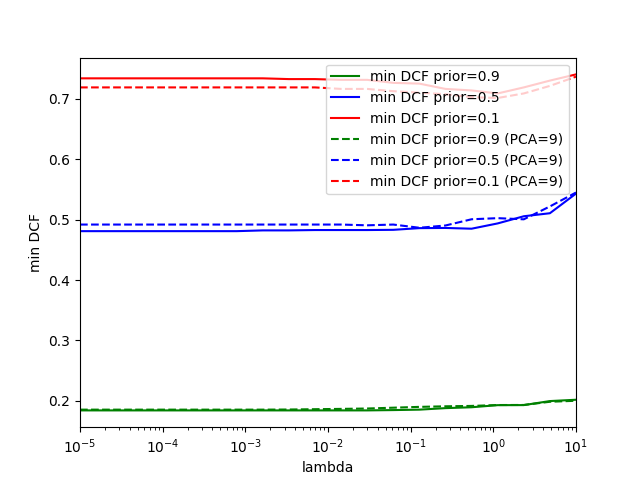
\includegraphics[scale=0.5]{../../images/LR_PCA_minDCF_comparison.png}
    \caption{DCF - Linear LogReg}
    \label{DCF - Linear LogReg}
\end{figure}

The figure 2.1 shows that using a $\lambda$ = 10\textsuperscript{-5} or $\lambda$ = 10\textsuperscript{-1}
is more or less the same, the minDCF doesn't change that much. From $\lambda$ = 10\textsuperscript{-1} to
+$\infty$ the minDCF will be too high.

For our main application, it's hard to see, but $\lambda$ = 0.4 is the best choice.

\begin{table}[H]
    \centering
    
    \begin{tabular}{lllllll}
        \hline
                                & pi=0.1 & pi=0.5 & pi=0.9 \\ \hline
                                & \multicolumn{3}{c}{NO-PCA}  \\
    Log Reg ($\lambda$ = 0.4)   & 0.715      & 0.485      & 0.189      \\
                                & \multicolumn{3}{c}{PCA m=9}  \\
    Log Reg ($\lambda$ = 0.4)   & 0.705      & 0.496       & 0.193       \\
                                & \multicolumn{3}{c}{PCA m=8}  \\
    Log Reg ($\lambda$ = 0.4)   & 0.689       & 0.483       & 0.188       \\
    \hline
    \end{tabular}
\end{table}

Overall the MVG without PCA has a \textbf{minDCF = 0.331} and this value is better than all 
the Linear Logistic Regression values (for our main application)

\clearpage

\subsection{Quadratic Logistic Regression}

The figure 2.2 shows how minDCF is affected by different values of $\lambda$. Also in this case, for
our main application, taking a $\lambda$=10\textsuperscript{-5} or $\lambda$=10\textsuperscript{-1}
doesn't change the minDCF that much.

\begin{figure}[H]
    \centering
    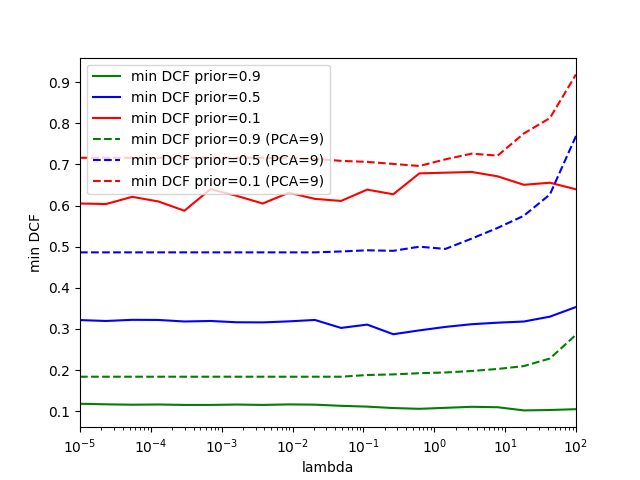
\includegraphics[scale=0.5]{../../images/QUAD_LR_PCA_minDCF_comparison.png}
    \caption{DCF - Linear LogReg}
    \label{DCF - Linear LogReg}
\end{figure}

It is also easy to see that PCA is pretty useless for all applications.
The minDCF it's always worse than the model without PCA.

\begin{table}[H]
    \centering
    
    \begin{tabular}{lllllll}
        \hline
                                & pi=0.1 & pi=0.5 & pi=0.9 \\ \hline
                                & \multicolumn{3}{c}{NO-PCA}  \\
    Log Reg ($\lambda$ = 0.4, $\pi$\textsubscript{T} = 0.1)   & 0.6      & 0.31      & 0.119      \\
    Log Reg ($\lambda$ = 0.4, $\pi$\textsubscript{T} = 0.5)   & 0.644      & 0.305      & 0.106       \\
    Log Reg ($\lambda$ = 0.4, $\pi$\textsubscript{T} = 0.9)   & 0.707      & 0.335      & 0.105      \\
                                & \multicolumn{3}{c}{PCA m=9}  \\ \hline
    Log Reg ($\lambda$ = 0.4, $\pi$\textsubscript{T} = 0.1)   & 0.691      & 0.489       & 0.189       \\
    Log Reg ($\lambda$ = 0.4, $\pi$\textsubscript{T} = 0.5)   & 0.7      & 0.497      & 0.191      \\
    Log Reg ($\lambda$ = 0.4, $\pi$\textsubscript{T} = 0.9)   & 0.713      & 0.506      & 0.194      \\
                                & \multicolumn{3}{c}{PCA m=8}  \\ \hline
    Log Reg ($\lambda$ = 0.4, $\pi$\textsubscript{T} = 0.1)   & 0.691       & 0.483       & 0.191       \\
    Log Reg ($\lambda$ = 0.4, $\pi$\textsubscript{T} = 0.5)   & 0.691      & 0.483      & 0.191      \\
    Log Reg ($\lambda$ = 0.4, $\pi$\textsubscript{T} = 0.9)   & 0.691      & 0.483      & 0.191      \\
    \hline
    \end{tabular}
\end{table}

This kind of model, with a Quadratic Kernel outperforms the MVG models, for our main application.

\clearpage

\section{Support Vector Machine}

In this section we are going to see how Linear SVM, Polynomial SVM and RBF SVM will handle our application

$\newline$
\textbf{SVM - Linear - Raw Feature}

$\newline$
\textbf{Linear SVM} can be obtained by the minimization of the primal problem:
\[\hat{J}(\hat{w}) = \frac{1}{2}||\hat{w}||^2 + C\sum_{i=1}^{n}max_i(0,1-z_i(\hat{w}^T\hat{x_i}))\]
where
\[\hat{x_i} = \biggl[ \hat{x_i} K \biggr] , \hat{w_i} = \biggl[w b\biggr]\]
and K is a regularization term.
\begin{figure}[h!]
    \centering
    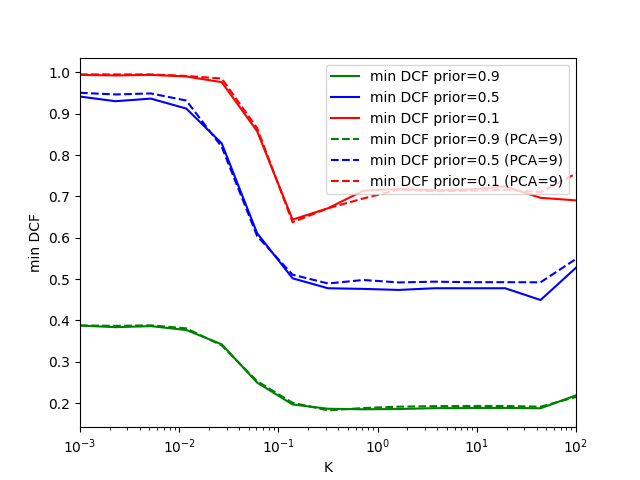
\includegraphics[scale = 0.5]{../../images/SVM_minDCF_comparison_C=1.png}
    \caption{Linear SVM with C=1}
\end{figure}

From Figure 2.3 we can see how K is affected (using C = 1). It can be seen that values of 
K between $10^{-1}$ and $10^{1}$ have a low DCF. In our cases we are going to try 3 different 
values of \(K = [0.1, 1, 10]\).

\begin{figure}[h!]
    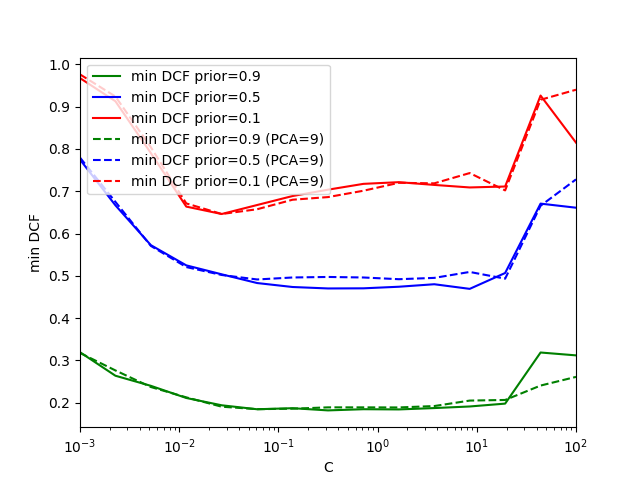
\includegraphics[scale = 0.5]{../../images/SVM_minDCF_comparison_K=1.png}
    \centering
    \caption{Linear SVM with K=1}
\end{figure}

Figure 2.4 shows the different values of C while setting K = 1. Again, it can be seen that the 
optiomal values of C are the ones between $10^{-1}$ and $10^{1}$. We are going to test 4 different 
values of \(C = [0.01, 0.1, 1, 10]\). We also decided to test 0.01 even if the minDCF is "optimal" only
for the $\pi$ = 0.1 

Here the table containing the results:

\begin{table}[H]
    \centering
    
    \begin{tabular}{ll|lllll}
        \hline
                                & &         K = 0.1 & K = 1.0 & K = 10 \\ \hline
                                & & \multicolumn{3}{c}{$\pi$=0.1} \\ \hline
                                & C = 0.01   & 0.99 & 0.68 & 0.71   \\
                                & C = 0.1    & 0.964 & 0.672 & 0.713  \\
                                & C = 1.0    & 0.67 & 0.722 & 0.715    \\
                                & C = 10.0   & 0.956 & 0.71 & 0.7  \\ \hline

                                & & \multicolumn{3}{c}{$\pi$=0.5} \\ \hline
                                & C = 0.01   & 0.921 & 0.532 & 0.473   \\
                                & C = 0.1    & 0.78 & 0.476 & 0.479  \\
                                & C = 1.0    & $\color{red}0.532$ & $\color{red}0.466$ & 0.473    \\
                                & C = 10.0   & 0.666 & 0.492 & $\color{red}0.47$  \\ \hline

                                & & \multicolumn{3}{c}{$\pi$=0.9} \\ \hline
                                & C = 0.01   & 0.379 & 0.216 & 0.187  \\
                                & C = 0.1    & 0.321 & 0.186 & 0.188  \\
                                & C = 1.0    & 0.216 & 0.184 & 0.188    \\
                                & C = 10.0   & 0.263 & 0.197 & 0.187  \\ 
    \hline
    \end{tabular}
\end{table}
$\newline$
\textbf{SVM - Linear - PCA with m = 9}

$\newline$
We also tried to apply PCA with m = 9 since from Figure 2.3 and Figure 2.4 we can see that
we can achive also a good minDCF.

\begin{table}[H]
    \centering
    
    \begin{tabular}{ll|lllll}
        \hline
                                & &         K = 0.1 & K = 1.0 & K = 10 \\ \hline
                                & & \multicolumn{3}{c}{$\pi$=0.1} \\ \hline
                                & C = 0.01   & 0.991 & 0.704 & 0.701    \\
                                & C = 0.1    & 0.971 & 0.669 & 0.718  \\
                                & C = 1.0    & 0.694 & 0.709 & 0.709    \\
                                & C = 10.0   & 0.685 & 0.672 & 0.73  \\ \hline

                                & & \multicolumn{3}{c}{$\pi$=0.5} \\ \hline
                                & C = 0.01   & 0.973 & 0.538 & 0.496   \\
                                & C = 0.1    & 0.776 & 0.493 & 0.492  \\
                                & C = 1.0    & 0.54 & 0.494 & $\color{red}0.489$    \\
                                & C = 10.0   & $\color{red}0.518$ & $\color{red}0.491$ & 0.492  \\ \hline

                                & & \multicolumn{3}{c}{$\pi$=0.9} \\ \hline
                                & C = 0.01   & 0.382 & 0.216 & 0.187  \\
                                & C = 0.1    & 0.321 & 0.182 & 0.191  \\
                                & C = 1.0    & 0.214 & 0.19 & 0.194    \\
                                & C = 10.0   & 0.223 & 0.196 & 0.195  \\ 
    \hline
    \end{tabular}
\end{table}

From this results we can conclude that using or not using PCA (with m = 9, so with almost all
features) doesn't change that much.

\newpage
\textbf{SVM - Quadratic - Raw Feature with degree = 2}

\begin{table}[H]
    \centering
    
    \begin{tabular}{ll|lllll}
        \hline
                                &  $\textbf{Constant = 0}$       & K = 0.1 & K = 1.0 & K = 10 \\ \hline
                                & & \multicolumn{3}{c}{$\pi$=0.1} \\ \hline
                                & C = 0.01   & 0.71 & 0.704 & 0.682    \\
                                & C = 0.1    & 0.713 & 0.674 & 0.678  \\
                                & C = 1.0    & 0.831 & 0.922 & 0.84    \\
                                & C = 10.0   & 0.982 & 0.994 & 0.975  \\ \hline

                                & & \multicolumn{3}{c}{$\pi$=0.5} \\ \hline
                                & C = 0.01   & 0.337 & 0.346 & 0.342   \\
                                & C = 0.1    & 0.324 & 0.344 & 0.346  \\
                                & C = 1.0    & 0.528 & 0.551 & 0.49    \\
                                & C = 10.0   & 0.947 & 0.957 & 0.946  \\ \hline

                                & & \multicolumn{3}{c}{$\pi$=0.9} \\ \hline
                                & C = 0.01   & 0.123 & 0.121 & 0.187  \\
                                & C = 0.1    & 0.125 & 0.11 & 0.115  \\
                                & C = 1.0    & 0.21 & 0.203 & 0.223    \\
                                & C = 10.0   & 0.586 & 0.769 & 0.583  \\ 
    \hline
    \end{tabular}
\end{table}

\begin{table}[H]
    \centering
    
    \begin{tabular}{ll|lllll}
        \hline
                                & $\textbf{Constant = 1}$      & K = 0.1 & K = 1.0 & K = 10 \\ \hline
                                & & \multicolumn{3}{c}{$\pi$=0.1} \\ \hline
                                & C = 0.01   & 0.63 & 0.623 & 0.598    \\
                                & C = 0.1    & 0.66 & 0.624 & 0.677  \\
                                & C = 1.0    & 0.96 & 0.931 & 0.95    \\
                                & C = 10.0   & 0.996 & 1.0 & 1.0  \\ \hline

                                & & \multicolumn{3}{c}{$\pi$=0.5} \\ \hline
                                & C = 0.01   & 0.316 & 0.311 & 0.313   \\
                                & C = 0.1    & 0.348 & 0.347 & 0.323  \\
                                & C = 1.0    & 0.701 & 0.631 & 0.644    \\
                                & C = 10.0   & 0.966 & 1.0 & 1.0  \\ \hline

                                & & \multicolumn{3}{c}{$\pi$=0.9} \\ \hline
                                & C = 0.01   & 0.113 & 0.114 & 0.104  \\
                                & C = 0.1    & 0.114 & 0.112 & 0.11  \\
                                & C = 1.0    & 0.281 & 0.207 & 0.233    \\
                                & C = 10.0   & 0.656 & 0.647 & 0.569  \\ 
    \hline
    \end{tabular}
\end{table}

$\newline$
\textbf{SVM - Quadratic - PCA with m = 9 and degree = 2}

\begin{table}[H]
    \centering
    
    \begin{tabular}{ll|lllll}
        \hline
                                & $\textbf{Constant = 0}$  &         K = 0.1 & K = 1.0 & K = 10 \\ \hline
                                & & \multicolumn{3}{c}{$\pi$=0.1} \\ \hline
                                & C = 0.01   & 0.645 & 0.645 & 0.638    \\
                                & C = 0.1    & 0.659 & 0.659 & 0.656  \\
                                & C = 1.0    & 0.92 & 0.871 & 0.916    \\
                                & C = 10.0   & 1.0 & 0.985 & 0.99  \\ \hline

                                & & \multicolumn{3}{c}{$\pi$=0.5} \\ \hline
                                & C = 0.01   & 0.331 & 0.344 & 0.354   \\
                                & C = 0.1    & 0.345 & 0.345 & 0.391  \\
                                & C = 1.0    & 0.449 & 0.575 & 0.574    \\
                                & C = 10.0   & 1.0 & 0.975 & 0.951  \\ \hline

                                & & \multicolumn{3}{c}{$\pi$=0.9} \\ \hline
                                & C = 0.01   & 0.127 & 0.124 & 0.109  \\
                                & C = 0.1    & 0.125 & 0.113 & 0.125  \\
                                & C = 1.0    & 0.181 & 0.203 & 0.172    \\
                                & C = 10.0   & 0.605 & 0.66 & 0.527  \\ 
    \hline
    \end{tabular}
\end{table}

\begin{table}[H]
    \centering
    
    \begin{tabular}{ll|lllll}
        \hline
                                & $\textbf{Constant = 1}$ &         K = 0.1 & K = 1.0 & K = 10 \\ \hline
                                & & \multicolumn{3}{c}{$\pi$=0.1} \\ \hline
                                & C = 0.01   & 0.576 & 0.584 & 0.59    \\
                                & C = 0.1    & 0.586 & 0.624 & 0.667  \\
                                & C = 1.0    & 0.894 & 0.992 & 0.975    \\
                                & C = 10.0   & 0.998 & 1.0 & 0.982  \\ \hline

                                & & \multicolumn{3}{c}{$\pi$=0.5} \\ \hline
                                & C = 0.01   & 0.335 & 0.334 & 0.306   \\
                                & C = 0.1    & 0.35 & 0.302 & 0.346  \\
                                & C = 1.0    & 0.688 & 0.772 & 0.56    \\
                                & C = 10.0   & 0.993 & 1.0 & 0.975  \\ \hline

                                & & \multicolumn{3}{c}{$\pi$=0.9} \\ \hline
                                & C = 0.01   & 0.118 & 0.117 & 0.105  \\
                                & C = 0.1    & 0.132 & 0.114 & 0.107  \\
                                & C = 1.0    & 0.22 & 0.236 & 0.189    \\
                                & C = 10.0   & 0.677 & 0.67 & 0.594  \\ 
    \hline
    \end{tabular}
\end{table}

$\newline$
\textbf{SVM - Quadratic - PCA with m = 8 and degree = 2}

\begin{table}[H]
    \centering
    
    \begin{tabular}{ll|lllll}
        \hline
                                & \textbf{Constant = 0} &         K = 0.1 & K = 1.0 & K = 10 \\ \hline
                                & & \multicolumn{3}{c}{$\pi$=0.1} \\ \hline
                                & C = 0.01   & 0.624 & 0.654 & 0.666    \\
                                & C = 0.1    & 0.66 & 0.648 & 0.658  \\
                                & C = 1.0    & 0.848 & 0.989 & 0.798    \\
                                & C = 10.0   & 0.981 & 0.999 & 0.97  \\ \hline

                                & & \multicolumn{3}{c}{$\pi$=0.5} \\ \hline
                                & C = 0.01   & 0.324 & 0.331 & 0.333   \\
                                & C = 0.1    & 0.321 & 0.336 & 0.317  \\
                                & C = 1.0    & 0.593 & 0.934 & 0.494    \\
                                & C = 10.0   & 0.97 & 0.999 & 0.91  \\ \hline

                                & & \multicolumn{3}{c}{$\pi$=0.9} \\ \hline
                                & C = 0.01   & 0.127 & 0.12 & 0.113  \\
                                & C = 0.1    & 0.124 & 0.11 & 0.116  \\
                                & C = 1.0    & 0.285 & 0.359 & 0.203    \\
                                & C = 10.0   & 0.511 & 0.74 & 0.563  \\ 
    \hline
    \end{tabular}
\end{table}

\begin{table}[H]
    \centering
    
    \begin{tabular}{ll|lllll}
        \hline
                                & \textbf{Constant = 1} &         K = 0.1 & K = 1.0 & K = 10 \\ \hline
                                & & \multicolumn{3}{c}{$\pi$=0.1} \\ \hline
                                & C = 0.01   & 0.561 & 0.541 & 0.53    \\
                                & C = 0.1    & 0.546 & 0.592 & 0.634  \\
                                & C = 1.0    & 0.985 & 0.865 & 0.98    \\
                                & C = 10.0   & 1.0 & 0.996 & 0..994  \\ \hline

                                & & \multicolumn{3}{c}{$\pi$=0.5} \\ \hline
                                & C = 0.01   & 0.323 & 0.32 & 0.308   \\
                                & C = 0.1    & 0.349 & 0.316 & 0.336  \\
                                & C = 1.0    & 0.657 & 0.649 & 0.7    \\
                                & C = 10.0   & 1.0 & 0.985 & 0.989  \\ \hline

                                & & \multicolumn{3}{c}{$\pi$=0.9} \\ \hline
                                & C = 0.01   & 0.114 & 0.108 & 0.101  \\
                                & C = 0.1    & 0.111 & 0.113 & 0.102  \\
                                & C = 1.0    & 0.262 & 0.217 & 0.211    \\
                                & C = 10.0   & 0.697 & 0.743 & 0.647  \\
    \hline
    \end{tabular}
\end{table}

\newpage
\textbf{SVM - Radial Basis kernel Function - Raw Feature}

\begin{table}[H]
    \centering
    
    \begin{tabular}{ll|lllll}
        \hline
                                & \textbf{$\gamma$ = 0.001} &         K = 0.1 & K = 1.0 & K = 10 \\ \hline
                                & & \multicolumn{3}{c}{$\pi$=0.1} \\ \hline
                                & C = 1.0    & 0.592 & 0.575 & 0.578    \\
                                & C = 10.0   & 0.58 & 0.599 & 0.601  \\
                                & C = 100.0   & 0.586 & 0.579 & 0.601  \\ \hline

                                & & \multicolumn{3}{c}{$\pi$=0.5} \\ \hline
                                & C = 1.0    & 0.302 & 0.3 & 0.301    \\
                                & C = 10.0   & 0.293 & 0.298 & 0.302  \\
                                & C = 100.0   & 0.332 & 0.331 & 0.335  \\ \hline

                                & & \multicolumn{3}{c}{$\pi$=0.9} \\ \hline
                                & C = 1.0    & 0.097 & 0.1 & 0.101    \\
                                & C = 10.0   & 0.089 & 0.089 & 0.089  \\
                                & C = 100.0   & 0.101 & 0.103 & 0.102  \\ 
    \hline
    \end{tabular}
\end{table}


\begin{table}[H]
    \centering
    
    \begin{tabular}{ll|lllll}
        \hline
                                & \textbf{$\gamma$ = 0.0001} &         K = 0.1 & K = 1.0 & K = 10 \\ \hline
                                & & \multicolumn{3}{c}{$\pi$=0.1} \\ \hline
                                & C = 1.0    & 0.671 & 0.662 & 0.659    \\
                                & C = 10.0   & 0.574 & 0.58 & 0.584  \\
                                & C = 100.0   & 0.568 & 0.575 & 0.725  \\ \hline

                                & & \multicolumn{3}{c}{$\pi$=0.5} \\ \hline
                                & C = 1.0    & 0.473 & 0.42 & 0.419    \\
                                & C = 10.0   & 0.406 & 0.381 & 0.354  \\
                                & C = 100.0   & 0.289 & 0.306 & 0.472  \\ \hline

                                & & \multicolumn{3}{c}{$\pi$=0.9} \\ \hline
                                & C = 1.0    & 0.163 & 0.159 & 0.158    \\
                                & C = 10.0   & 0.137 & 0.133 & 0.13  \\
                                & C = 100.0   & 0.097 & 0.103 & 0.276  \\ 
    \hline
    \end{tabular}
\end{table}

$\newline$
\textbf{SVM - Radial Basis kernel Function - PCA with m=9}


\begin{table}[H]
    \centering
    
    \begin{tabular}{ll|lllll}
        \hline
                                & \textbf{$\gamma$ = 0.001} &         K = 0.1 & K = 1.0 & K = 10 \\ \hline
                                & & \multicolumn{3}{c}{$\pi$=0.1} \\ \hline
                                & C = 1.0    & 0.588 & 0.585 & 0.579    \\
                                & C = 10.0   & 0.534 & 0.541 & 0.542  \\
                                & C = 100.0   & 0.678 & 0.671 & 0.906  \\ \hline

                                & & \multicolumn{3}{c}{$\pi$=0.5} \\ \hline
                                & C = 1.0    & 0.295 & 0.294 & 0.298    \\
                                & C = 10.0   & 0.297 & 0.301 & 0.299  \\
                                & C = 100.0   & 0.328 & 0.333 & 0.895  \\ \hline

                                & & \multicolumn{3}{c}{$\pi$=0.9} \\ \hline
                                & C = 1.0    & 0.103 & 0.104 & 0.104    \\
                                & C = 10.0   & 0.102 & 0.103 & 0.102  \\
                                & C = 100.0   & 0.107 & 0.108 & 0.285  \\ 
    \hline
    \end{tabular}
\end{table}


\begin{table}[H]
    \centering
    
    \begin{tabular}{ll|lllll}
        \hline
                                & \textbf{$\gamma$ = 0.0001} &         K = 0.1 & K = 1.0 & K = 10 \\ \hline
                                & & \multicolumn{3}{c}{$\pi$=0.1} \\ \hline
                                & C = 1.0    & 0.672 & 0.672 & 0.662    \\
                                & C = 10.0   & 0.621 & 0.605 & 0.624  \\
                                & C = 100.0   & 0.553 & 0.502 & 0.592  \\ \hline

                                & & \multicolumn{3}{c}{$\pi$=0.5} \\ \hline
                                & C = 1.0    & 0.439 & 0.433 & 0.42    \\
                                & C = 10.0   & 0.407 & 0.391 & 0.376  \\
                                & C = 100.0   & 0.301 & 0.302 & 0.317  \\ \hline

                                & & \multicolumn{3}{c}{$\pi$=0.9} \\ \hline
                                & C = 1.0    & 0.165 & 0.159 & 0.16    \\
                                & C = 10.0   & 0.139 & 0.132 & 0.128  \\
                                & C = 100.0   & 0.103 & 0.106 & 0.12  \\ 
    \hline
    \end{tabular}
\end{table}

$\newline$
\textbf{SVM - Radial Basis kernel Function - PCA with m=8}


\begin{table}[H]
    \centering
    
    \begin{tabular}{ll|lllll}
        \hline
                                & \textbf{$\gamma$ = 0.001} &         K = 0.1 & K = 1.0 & K = 10 \\ \hline
                                & & \multicolumn{3}{c}{$\pi$=0.1} \\ \hline
                                & C = 1.0    & 0.568 & 0.569 & 0.573    \\
                                & C = 10.0   & 0.528 & 0.54 & 0.545  \\
                                & C = 100.0   & 0.664 & 0.672 & 0.666  \\ \hline

                                & & \multicolumn{3}{c}{$\pi$=0.5} \\ \hline
                                & C = 1.0    & 0.297 & 0.297 & 0.296    \\
                                & C = 10.0   & 0.281 & 0.29 & 0.294  \\
                                & C = 100.0   & 0.318 & 0.315 & 0.305  \\ \hline

                                & & \multicolumn{3}{c}{$\pi$=0.9} \\ \hline
                                & C = 1.0    & 0.102 & 0.104 & 0.105    \\
                                & C = 10.0   & 0.101 & 0.103 & 0.103  \\
                                & C = 100.0   & 0.108 & 0.105 & 0.104  \\ 
    \hline
    \end{tabular}
\end{table}


\begin{table}[H]
    \centering
    
    \begin{tabular}{ll|lllll}
        \hline
                                & \textbf{$\gamma$ = 0.0001} &         K = 0.1 & K = 1.0 & K = 10 \\ \hline
                                & & \multicolumn{3}{c}{$\pi$=0.1} \\ \hline
                                & C = 1.0    & 0.665 & 0.662 & 0.645    \\
                                & C = 10.0   & 0.617 & 0.607 & 0.679  \\
                                & C = 100.0   & 0.55 & 0.529 & 0.844  \\ \hline

                                & & \multicolumn{3}{c}{$\pi$=0.5} \\ \hline
                                & C = 1.0    & 0.439 & 0.433 & 0.43    \\
                                & C = 10.0   & 0.397 & 0.389 & 0.387  \\
                                & C = 100.0   & 0.306 & 0.29 & 0.686  \\ \hline

                                & & \multicolumn{3}{c}{$\pi$=0.9} \\ \hline
                                & C = 1.0    & 0.165 & 0.158 & 0.156    \\
                                & C = 10.0   & 0.141 & 0.135 & 0.153  \\
                                & C = 100.0   & 0.106 & 0.107 & 0.301  \\ 
    \hline
    \end{tabular}
\end{table}

\clearpage

\section{Gaussian Misxture Models}

$\newline$
\textbf{GMM - RAW Feature}


\begin{table}[H]
    \centering
    
    \begin{tabular}{ll|lllllll}
        \hline
                                & \textbf{Components} & $2^1$ & $2^2$ & $2^3$ & $2^4$ & $2^5$ & $2^6$ & $2^7$ \\ \hline
                                & & \multicolumn{7}{c}{$\pi$=0.1} \\ \hline
                                & Full-Cov        & 0.497 & 0.526 & 0.69 & 0.63 & 0.877 & 0.976 & 1.0   \\
                                & Diag-Cov        & 0.719 & 0.544 & 0.514 & 0.531 & 0.592 & 0.698 & 0.741  \\
                                & Full-Cov-Tied   & 0.616 & 0.611 & 0.558 & 0.542 & 0.588 & 0.563 & 0.71  \\ 
                                & Diag-Cov-Tied   & 0.805 & 0.558 & 0.501 & 0.56 & 0.601 & 0.673 & 0.765  \\ \hline

                                & & \multicolumn{7}{c}{$\pi$=0.5} \\ \hline
                                & Full-Cov          & 0.28 & 0.264 & 0.325 & 0.391 & 0.568 & 0.737 & 1.0     \\
                                & Diag-Cov          & 0.451 & 0.275 & 0.262 & 0.26 & 0.281 & 0.359 & 0.425  \\
                                & Full-Cov-Tied     & 0.331 & 0.255 & 0.244 & 0.253 & 0.292 & 0.314 & 0.341  \\ 
                                & Diag-Cov-Tied     & 0.462 & 0.276 & 0.254 & 0.262 & 0.282 & 0.286 &  0.358 \\ \hline

                                & & \multicolumn{7}{c}{$\pi$=0.9} \\ \hline
                                & Full-Cov          & 0.105 & 0.094 & 0.108 & 0.124 & 0.213 & 0.306 & 0.523    \\
                                & Diag-Cov          & 0.141 & 0.087 & 0.09 & 0.092 & 0.107 & 0.122 & 0.144  \\
                                & Full-Cov-Tied     & 0.111 & 0.098 & 0.083 & 0.087 & 0.104 & 0.108 & 0.134  \\ 
                                & Diag-Cov-Tied     & 0.144 & 0.086 & 0.089 & 0.088 & 0.093 & 0.11 & 0.131  \\ \hline 
    \hline
    \end{tabular}
\end{table}

$\newline$
\textbf{GMM - PCA with m = 9}


\begin{table}[H]
    \centering
    
    \begin{tabular}{ll|lllllll}
        \hline
                                & \textbf{Components} & $2^1$ & $2^2$ & $2^3$ & $2^4$ & $2^5$ & $2^6$ & $2^7$ \\ \hline
                                & & \multicolumn{7}{c}{$\pi$=0.1} \\ \hline
                                & Full-Cov          & 0.455 & 0.599 & 0.599 & 0.684 & 0.837 & 0.999 & 1.0    \\
                                & Diag-Cov          & 0.742 & 0.599 & 0.553 & 0.546 & 0.513 & 0.638 & 0.729  \\
                                & Full-Cov-Tied     & 0.629 & 0.608 & 0.56 & 0.56 & 0.494 & 0.522 & 0.589  \\ 
                                & Diag-Cov-Tied     & 0.741 & 0.554 & 0.528 & 0.538 & 0.554 & 0.58 & 0.624  \\ \hline

                                & & \multicolumn{7}{c}{$\pi$=0.5} \\ \hline
                                & Full-Cov          & 0.299 & 0.293 & 0.322 & 0.371 & 0.467 & 0.704 & 1.0    \\
                                & Diag-Cov          & 0.367 & 0.272 & 0.253 & 0.281 & 0.287 & 0.34 & 0.374  \\
                                & Full-Cov-Tied     & 0.33 & 0.261 & 0.269 & 0.254 & 0.285 & 0.324 & 0.322  \\ 
                                & Diag-Cov-Tied     & 0.368 & 0.268 & 0.248 & 0.276 & 0.306 & 0.328 & 0.359  \\ \hline

                                & & \multicolumn{7}{c}{$\pi$=0.9} \\ \hline
                                & Full-Cov          & 0.099 & 0.091 & 0.113 & 0.125 & 0.158 & 0.218 & 0.376   \\
                                & Diag-Cov          & 0.114 & 0.096 & 0.094 & 0.093 & 0.103 & 0.109 & 0.135 \\
                                & Full-Cov-Tied     & 0.109 & 0.103 & 0.087 & 0.095 & 0.109 & 0.119 & 0.138  \\ 
                                & Diag-Cov-Tied     & 0.114 & 0.087 & 0.095 & 0.09 & 0.093 & 0.101 &  0.12 \\ \hline 
    \hline
    \end{tabular}
\end{table}


\end{document}